\section{Fallbeispiel Zoo – Ein erstes Domänenklassendiagramm}
\label{sec:Kap-3.3}

Folgende Situation: Sie haben Ihr Informatik- (wahlweise Wirtschaftsinformatik-) Studium abgeschlossen und Ihre erste Stelle in einem Unternehmen angetreten, das Softwarelösungen für kleine und mittelständische Betriebe entwickelt. Die Kollegin, mit der Sie sich ein Büro teilen, ist erkrankt. Daher schickt Ihr Chef, Herr Steiber, Sie an ihrer Stelle zu einem Gespräch mit Frau Dr. Walther.

\minisec{Ihr Auftrag}

Hr. Steiber: „Frau Dr. Walther ist die Direktorin des Zoos hier in der Stadt – und eine gute Bekannte von mir. Sie ist vor einigen Wochen auf mich zugekommen, da sie vielleicht – so ganz sicher ist sie da offensichtlich noch nicht – eine Zoo-Verwaltungssoftware benötigt. Ich hatte Frau Schwaber, Ihre leider kranke Kollegin, gebeten mit ihr heute ein erstes informelles Gespräch zu führen. Das müssen Sie jetzt übernehmen. Wir haben noch nie einen Zoo als Kunden gehabt und die Domäne Zoo ist uns allen hier nicht wirklich bekannt. Lassen Sie sich von Frau Dr. Walther etwas über die Domäne erzählen, und auch für welche Aufgaben sie ein Softwaresystem benötigen würde – wobei, wie gesagt, ich vermute, dass sie das selber noch nicht genau weiß. Für uns als Firma wäre es wichtig, dass wir einschätzen können, ob es sich lohnt, außer diesem ersten Informationsgespräch weitere Ressourcen zu investieren und auf eine Auftragserteilung hinzuarbeiten. Daher darf das zu lösende Problem nicht zu klein sein – ich sag mal, nur eine Eingabemaske zu erstellen, in der Frau Dr. Walther die Namen der Tiere eingeben kann, ist für uns nicht interessant. Auf der anderen Seite können wir mit unserem doch recht kleinen Team natürlich auch keine allumfassende Automatisierung sämtlicher Zoo-Abläufe liefern. Daher, versuchen Sie so viele Informationen über die Problemdomäne zu erhalten wie möglich. Erstellen Sie idealerweise auch im Anschluss an das Gespräch schon einmal einen ersten Entwurf eines Domänenklassendiagramms. Dann haben wir eine Diskussionsgrundlage für die Teambesprechung nächste Woche.“

\minisec{Ihr Gespräch mit der Zoodirektorin}

Fr. Walther: „Hallo, herzlich willkommen. Herr Steiber hat mich schon informiert, dass Sie Ihre Kollegin vertreten. Er sagt, ich soll Ihnen etwas über unseren Zoo erzählen – das ist kein Problem. Außerdem meinte er, ich solle schon einmal überlegen, was eine Zoo-Software können muss. Woher soll ich das wissen? Sie sind doch die Experten in der Softwareentwicklung. Sie wissen viel besser, was Softwareprodukte können müssen. Also, unser Zoo: Wir haben jährlich ca. 150.000 Besucher, im Jahresverlauf ist die Besucherzahl stark schwankend. 80 Prozent unserer Besucher sind Kinder. Natürlich hat irgendwie jedes Kind sein eigenes Lieblingstier, was sie aber alle auch mögen ist unser Streichelzoo. Da haben wir nicht nur die üblichen Kaninchen, Meerschweinchen, Ziegen und Schafe, sondern auch unser Warzenschwein Rudi. Rudi war das erste Tier, für das wir vor ein paar Jahren die Möglichkeit eingerichtet haben, für einen jeweils begrenzten Zeitraum eine Patenschaft zu übernehmen. Mittlerweile existieren weitere Patenschaften für vier unserer Schlangen, unsere zwei Axolotl und den Kormoran. Eigentlich möchten wir das Patenschaftssystem auf alle unsere Tiere ausweiten und auch die Möglichkeit unterschiedlich langer Patenschaften bieten, aber ohne technische Unterstützung ist der Verwaltungsaufwand zu hoch. Kinder, die eine Patenschaft übernommen haben, erhalten für diesen Zeitraum freien Eintritt in den Zoo und können an bestimmten Tagen beim Füttern ihres Patentiers helfen. Wir beschäftigen fünfzehn Tierpflegerinnen und Tierpfleger und einen Tierarzt als Angestellte. Oft reicht ein Tierarzt nicht aus, sodass wir in diesen Fällen externe Tierärzte beauftragen müssen, was so kurzfristig oft nicht immer einfach ist. Wir planen langfristig eine zweite feste Tierarztstelle im Zoo einzurichten, vor allem da wir aktuell unseren Tierbestand erweitern. Bisher haben wir 26 verschiedene Tierarten mit entsprechend vielen Unterarten, \zb haben wir drei verschiedene Affenarten im Zoo. Natürlich hat jedes Tier einen Namen, und wir versuchen immer die Besucher einzubinden, wenn ein neugeborenes Tier einen Namen benötigt. Da kommt dann auch mal Shaggy raus als Name für unsere gestern geborene Testudo Graeca. Wir würden gerne alle Informationen zu unseren Tieren – also wann sie geboren sind, wer die Eltern sind, wie alt sie werden können, was sie fressen, aus welchem Zoo sie gegebenenfalls ausgeliehen sind und wie lange und ganz vieles mehr – unseren Besuchern auch über das Internet zur Verfügung stellen, aber das ist sicher aufwändig. Andererseits könnte man dann vielleicht die Eintrittskarten auch gleich online verkaufen, vielleicht würden wir dann noch mehr Besucher bekommen. Wir nutzen schon ein Onlinesystem, wenn wir Käfige oder Tiere aus anderen Zoos für eine bestimmte Zeit ausleihen und eine Software, mit der wir die Dienstpläne und Aufgaben unserer Tierpfleger verwalten, das wär schon gut, wenn das alles ein System wäre. Wir möchten langfristig nur noch fest installierte Gehege für die Tiere haben, in denen sie auch genug Platz und artgerechte Bedingungen haben, aber im Moment müssen wir auch Tiere in Käfigen halten, da sich die Bauarbeiten für die Zoo-Erweiterung verzögern. Aber wenn das mal fertig ist, werden wir endlich auch Eisbären und Nashörner haben, da fragen die Besucher nach. Seit letztem Jahr haben wir zwei Giraffen, da erhoffen wir uns dieses Jahr Nachwuchs. Tja, was müssen Sie noch wissen über unseren Zoo? Ja, genau: wir haben auch mehrere Spielplätze und natürlich Eis- und Pizzastände. Die Essensstände haben wir verpachtet. Das läuft ganz gut. Um das Essen für die Tiere kümmern sich die jeweiligen Tierpfleger, die kaufen entsprechend ein. Das müsste man sich auch mal angucken, ob es nicht sinnvoller wäre, die Futterbestellungen zentral zu machen, das müsste doch mit Softwareunterstützung auch viel leichter zu realisieren sein, und dann könnten wir vielleicht auch gleich noch für die Besucher im Internet Informationen über die Tierpfleger zur Verfügung stellen. Gerade unsere Stammgäste mit den Jahreskarten finden es wichtig den Tierpfleger zu kennen, der ihr Lieblingstier versorgt. Haben Sie Fragen?“ 

Frau Dr. Walther hatte sich viel Zeit für das Gespräch genommen, sodass Sie nach ihren Ausführungen noch Fragen stellen konnten. Die Antworten auf die Nachfragen zu Objekten und Beziehungen der Domäne Zoo haben Sie, soweit es ging, direkt bei der Erstellung des Domänenklassendiagramms berücksichtigt. Abbildung~\ref{fig:entwurf_domaene_zoo} zeigt Ihren ersten Entwurf eines Domänenklassendiagramms für die Domäne Zoo. Für die Teambesprechung in der folgenden Woche, in der diskutiert werden soll, ob weitere Ressourcen in die Akquirierung dieses Auftrags fließen sollen, haben Sie außerdem eine Übersicht erstellt, aus welchen großen Teilsystemen eine allumfassende Zoo-Software nach Frau Dr. Walthers Vorstellungen Ihrer Ansicht nach bestehen würde. Zudem haben Sie eine lange Liste mit offenen Fragen zur Domäne Zoo angelegt, die mit Frau Dr. Walther geklärt werden müssten, bevor man mit der Beschreibung des Funktionsumfangs einer Zoo-Software beginnen könnte. Diese Arbeit haben Sie nicht vergebens investiert, wir werden uns damit in Lektion~4 % todo Lektion~\ref{sec:Lektion-4} 
beschäftigen. Aktuell betrachten wir aber nur Ihren Entwurf für ein Domänenklassendiagramm.

\minisec{Domänenklassendiagramm}

Ab dieser Stelle des Texts verlassen Sie Ihre Rolle als Berufseinsteiger(in) in einer Software-Firma und übernehmen wieder die Rolle als Studierende(r) des Kurses Softwareengineering. In Abbildung~\ref{fig:entwurf_domaene_zoo} finden Sie UML-Konzepte wieder, die wir in Kapitel~\ref{sec:Kap-3.2.4} behandelt haben:

% Die Grafik "Zoo" soll über die ganze Seite gehen.
% Versucht wird dies hier mit "\makebox[0pt]{\includegraphics...}".
%\begin{figure}[h!]
%	\centering
%	\makebox[0pt]{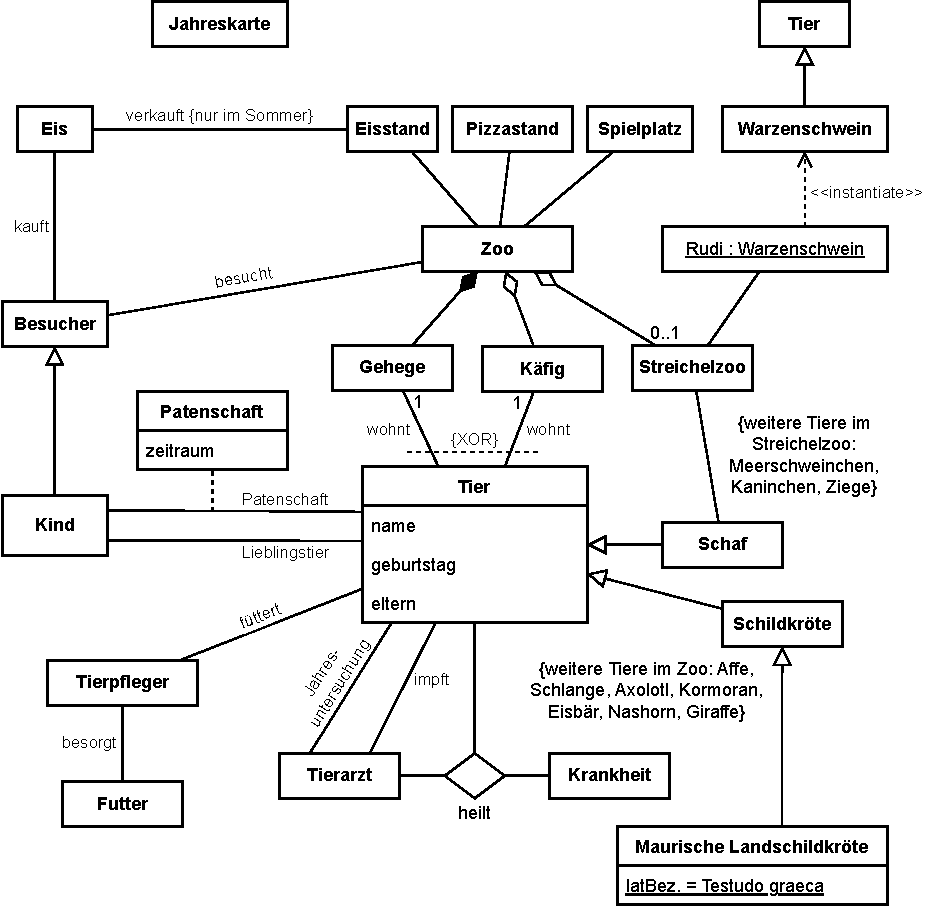
\includegraphics[width=0.9\paperwidth,height=0.9\paperheight,keepaspectratio]{Bilder/Kapitel-3/zoo.pdf}}
%	\caption{Ein erster Entwurf für ein Domänenklassendiagramm zur Domäne Zoo.}
%	\label{fig:entwurf_domaene_zoo}
%\end{figure}

\null\newpage
%\thispagestyle{empty}
\begin{textblock*}{\paperwidth}(0mm,4cm)
	\begin{figure}
		\centering
		\noindent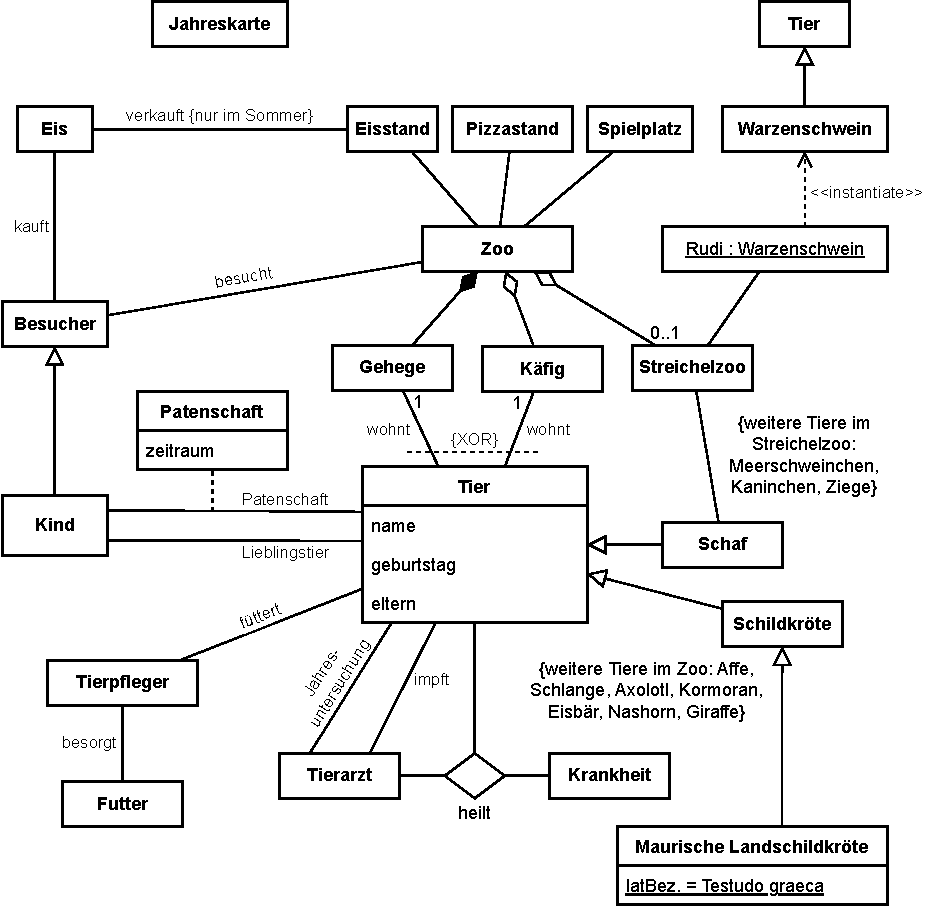
\includegraphics[width=0.95\paperwidth,height=\paperheight,keepaspectratio]{Bilder/Kapitel-3/zoo.pdf}
		\caption{Ein erster Entwurf für ein Domänenklassendiagramm zur Domäne Zoo.}
		\label{fig:entwurf_domaene_zoo}
	\end{figure}
\end{textblock*}
\null\newpage


\begin{itemize}
	\item Die Assoziationen zwischen \sttpUMLText{Tier} und \sttpUMLText{Gehege} sowie zwischen \sttpUMLText{Tier} und \sttpUMLText{Käfig} sind mit dem Zusatz \{XOR\} versehen, der modelliert, dass jedes Tier-Objekt entweder in einem Gehege oder in einem Käfig wohnt, aber nicht gleichzeitig in beiden.
	\item Die Beziehung zwischen \sttpUMLText{Zoo} und \sttpUMLText{Käfig} ist als Aggregation modelliert, da Käfige nach Frau Dr. Walthers Aussage aus anderen Zoos ausgeliehen werden können. Die Beziehung zwischen \sttpUMLText{Zoo} und \sttpUMLText{Gehege} ist dagegen als Komposition modelliert, da Gehege im Zoo fest installiert sind und nicht in einen anderen Zoo transportiert werden können. Der genaue Unterschied zwischen Gehege und Käfig ist uns aktuell noch nicht klar, dementsprechend müssen wir vermutlich später auch nochmal die Kompositions- bzw. Aggregations-Modellierung zur Klasse \sttpUMLText{Zoo} diskutieren.
	\item Die Maurische Landschildkröte ist als Spezialisierung einer Schildkröte und Letztere wiederum als Spezialisierung eines Tiers modelliert. In der Klasse \linebreak \sttpUMLText{Maurische Landschildkröte} finden Sie mit der lateinischen Bezeichnung für diese Tierart zudem ein Beispiel für ein sogenanntes Klassenattribut. Diese Art von Attributen lernen Sie in Lektion~4 % todo Lektion~\ref{sec:Lektion-4}
	kennen.
	\item Die Assoziation zwischen \sttpUMLText{Eisstand} und \sttpUMLText{Eis} zeigt ein Beispiel für eine textuelle Ergänzung zu einer Assoziation. Inhaltlich wird hier modelliert, dass die Eisstände nur während des Sommers Eis verkaufen. Ob die Eisstände im Winter etwas anderes verkaufen, einfach geschlossen sind oder aus dem Zoo entfernt werden, wissen wir nicht. Dementsprechend ist auch die Beziehung zwischen \sttpUMLText{Eisstand} und \sttpUMLText{Zoo} unklar. Aktuell ist nur modelliert, dass es eine Beziehung gibt, welcher Art (Assoziationsname) diese Beziehung ist, bleibt offen.
	\item Zwischen den Klassen \sttpUMLText{Tierarzt} und \sttpUMLText{Tier} gibt es mehrere Beziehungen. Mit der Assoziation \sttpUMLText{impft} wird modelliert, dass Tierärzte Tiere impfen. Die Assoziation \sttpUMLText{Jahresuntersuchung} modelliert, dass Tierärzte bei Tieren regelmäßige Vorsorgeuntersuchungen vornehmen. Üblicherweise verwendet man für Assoziationsnamen Verben. Der Assoziationsname \sttpUMLText{Jahresuntersuchung} ist ein Beispiel für einen Fall, in dem ein Nomen als Assoziationsname mal geeigneter ist als ein Verb.
\end{itemize}

Das Domänenklassendiagramm zeigt auch UML-Konstrukte, die Sie noch nicht kennengelernt haben. Neben den zwei eben angesprochenen Assoziationen ist die Klasse \sttpUMLText{Tierarzt} noch durch eine weitere Assoziation mit der Klasse \sttpUMLText{Tier} verbunden: Mit den durch eine Raute verknüpften Linien modelliert man in UML Beziehungen zwischen mehr als zwei Klassen, sogenannte \textit{n-äre Beziehungen}
\marginline{n-äre Beziehungen}
(\zb drei Klassen: ternär, vier Klassen: quaternär). In diesem Fall besteht eine Assoziation mit Namen \sttpUMLText{heilt} zwischen der Klasse \sttpUMLText{Tierarzt}, der Klasse \sttpUMLText{Tier} und der Klasse \sttpUMLText{Krankheit}. Damit wird ausgedrückt, dass Tierärzte Tiere von Krankheiten heilen. Java und viele andere objektorientierte Programmiersprachen unterstützen das Konzept der n-ären Beziehungen nicht, sodass bei der Implementierung solche Assoziationen in andere Formen von Assoziationen umgewandelt werden müssen. In Domänenmodellen können n-äre Beziehungen aber vorkommen, wenn sie in der Realwelt existieren (und dementsprechend den Domänenexperten geläufig sind), denn Domänenmodelle sollen noch unabhängig sein von jeglichen späteren Implementierungsbedürfnissen.

Zwischen den Klassen \sttpUMLText{Kind} und \sttpUMLText{Tier} bestehen ebenfalls mehrere Assoziationen. Die Assoziation \sttpUMLText{Lieblingstier} modelliert, dass Kinder Lieblingstiere unter den Zootieren haben können. Ob es sich dabei jeweils um genau ein Tier handelt, oder ob Kinder auch mehrere Lieblingstiere haben können, wissen wir zum jetzigen Zeitpunkt nicht, daher sind keine Multiplizitäten angegeben. Die Assoziation \sttpUMLText{Patenschaft} zwischen \sttpUMLText{Kind} und \sttpUMLText{Tier} ist unter Verwendung einer sogenannten \textit{Assoziationsklasse}
\marginline{Assoziationsklassen}
modelliert. Eine Assoziationsklasse bietet die Möglichkeit, eine Assoziation mit Merkmalen auszustatten. Man verwendet Assoziationsklassen, um Charakteristika abzubilden, die Teil der Beziehung zwischen den beteiligten Objekten sind und sich nicht einer der an der Beziehung beteiligten Klassen zuordnen lassen. In unserem Beispiel spielt für eine Patenschaft, die ein Kind für ein Tier übernimmt, der Zeitraum dieser Patenschaft eine Rolle. In der UML-Darstellung wird die Assoziationsklasse mit einer gestrichelten Linie an die Assoziationslinie angebunden. Der Name der Assoziationsklasse und der Name der Assoziation müssen identisch sein, wobei letzterer optional ist. Ähnlich wie bei den n-ären Beziehungen müssen Assoziationsklassen-Beziehungen für die Implementierung in andere Beziehungsformen umgewandelt werden, da die objektorientierten Programmiersprachen das Konzept der Assoziationsklasse nicht unterstützen. In Domänenmodellen sind sie aber häufig zu finden.

Ein  weiteres Konstrukt im Diagramm, auf das wir zuvor nur kurz verwiesen haben, ist die instantiate-Abhängigkeit.
\marginline{instantiate-Abhängigkeit}
Diese Darstellung wird verwendet, wenn man eine Klasse und ein Objekt dieser Klasse im selben Diagramm unterbringen möchte. In unserem Fall findet sich sowohl die Klasse \sttpUMLText{Warzenschwein} als auch das Objekt \sttpUMLText{Rudi} des Typs Warzenschwein im Diagramm. Der gestrichelte Pfeil mit der Angabe \sttpUMLText{<<instantiate>>} signalisiert, dass \sttpUMLText{Rudi} ein Objekt der Klasse \sttpUMLText{Warzenschwein} ist. In den meisten Fällen werden instantiate-Abhängigkeiten in Objektdiagrammen verwendet, um zu einer konkreten Objektkonstellation zusätzliche Informationen über die Klasse dieses Objekts zur Verfügung zu stellen. Die Modellierung eines Objekts innerhalb eines Klassendiagramms ist eher selten. Warum modelliert man \sttpUMLText{Rudi} überhaupt im Domänenklassendiagramm und nicht nur die Klasse \sttpUMLText{Warzenschwein}? Das Warzenschwein Rudi wurde von Frau Dr. Walther, auf deren Aussagen dieser Diagrammentwurf beruht, besonders hervorgehoben. Möglicherweise ist Rudi ein wichtiger Bestandteil der Domäne. Das können wir noch nicht einschätzen. Aktuell wissen wir zudem noch nicht, ob Warzenschweine grundsätzlich für einen Streichelzoo geeignet sind, oder ob das explizit nur für Rudi zutrifft, weil der ein besonders freundliches Exemplar seiner Art ist. Auf unserem bisherigen Wissensstand beruhend behandeln wir Rudi daher erst einmal als zu modellierenden Bestandteil der Domäne.

Oberhalb der Klasse \sttpUMLText{Warzenschwein} finden Sie im Diagramm eine zweite Klasse \sttpUMLText{Tier}. Nach UML-Definition ist damit dieselbe Klasse \sttpUMLText{Tier} wie in der Mitte des Diagramms gemeint. Die doppelte Darstellung der Tier-Klasse erfolgt hier aus Übersichtlichkeitsgründen, um die Generalisierungsverbindung zwischen der Warzenschwein- und der Tier-Klasse nicht über das ganze Diagramm ziehen zu müssen. Die mehrfache Darstellung von Klassen in einem Diagramm sollte man nur sehr dosiert anwenden, da die existierenden Beziehungen zwischen Klassen mit jeder Dopplung einer Klasse im Diagramm weniger gut zu überblicken sind.

Außer dem Warzenschwein Rudi sind im Diagramm bisher nur die Tierarten Schaf und Schildkröte modelliert. Aus Übersichtsgründen und auch weil wir noch nicht alle Tierarten kennen, wird auf weitere Tiere im Zoo und im Streichelzoo nur in Form textueller Ergänzungen zum Diagramm verwiesen. 

Oben links im Diagramm finden Sie die Klasse \sttpUMLText{Jahreskarte}, für die keine Beziehungen modelliert sind. Aktuell haben wir zu wenig Informationen, um der Klasse \sttpUMLText{Jahreskarte} einen Platz innerhalb der Domäne zuordnen zu können. Gleiches gilt für die Klassen \sttpUMLText{Pizzastand} und \sttpUMLText{Spielplatz}, die wohl irgendwie zum Zoo gehören – und so unspezifiziert haben wir sie auch modelliert –, über die wir ansonsten aber keine Aussagen treffen können. Aufgefallen ist Ihnen vermutlich auch, dass mit ganz wenigen Ausnahmen noch keine Multiplizitäten für die Assoziationen angegeben sind. Auch diese Informationen liegen uns nicht vor.

Wir  werden uns mit diesem Domänenklassendiagramm-Entwurf in der nächsten Kurseinheit noch ausführlicher beschäftigen. An dieser Stelle hören Sie schon einmal das Credo, das Sie im weiteren Verlauf des Kurses immer mal wieder zu hören bekommen: Die \textbf{eine} Wahrheit gibt es im Kontext von Modellierung nicht. Das Modellieren
\marginline{Modellieren ist subjektiv}
von Sachverhalten – seien es Realweltzusammenhänge oder Entwurfsentscheidungen für die Implementierung – ist stets eine subjektive Handlung. Von ganz trivialen Beispielen einmal abgesehen, können identische Sachverhalte von verschiedenen Modellierern also durchaus unterschiedlich modelliert werden. Es gibt durchaus Heuristiken, an denen man sich als Modellierer orientieren kann („üblicherweise“), aber keine Formel für das ideale Diagramm. Die UML unterstützt durch die mittlerweile recht ausgereifte inhaltliche Abgrenzung ihrer unterschiedlichen Modellierungselemente aber eine gewisse Standardisierung. 